\documentclass[UTF8,fontset=windows,11pt,a4paper]{ctexart}
\usepackage[margin=2.15cm]{geometry}
\usepackage{amsmath,amssymb,booktabs,tabularx,longtable,array,multirow}
\usepackage{graphicx,xcolor,enumitem,fancyhdr,hyperref,xurl,float,caption}
\graphicspath{{../figures/}}
\setCJKmonofont{SimSun}
\definecolor{ok}{RGB}{25,120,70}
\definecolor{pending}{RGB}{190,105,10}
\definecolor{bad}{RGB}{180,35,45}
\definecolor{blue}{RGB}{35,75,130}
\definecolor{shade}{RGB}{245,247,250}
\hypersetup{
  colorlinks=true,
  linkcolor=blue,
  urlcolor=blue,
  pdfauthor={FG-MEE validation workbench},
  pdftitle={FG-MEE Stage 2 deep validation and innovation report}
}
\pagestyle{fancy}
\fancyhf{}
\lhead{FG-MEE 深入验证与创新工况报告}
\rhead{2026-07-15}
\cfoot{\thepage}
\setlength{\headheight}{15pt}
\setlength{\parindent}{2em}
\setlength{\parskip}{0.28em}
\renewcommand{\arraystretch}{1.16}
\captionsetup{font=small,labelfont=bf}
\newcommand{\pass}{\textcolor{ok}{\textbf{完成}}}
\newcommand{\wait}{\textcolor{pending}{\textbf{待补齐}}}
\newcommand{\failure}{\textcolor{bad}{\textbf{未通过}}}
\newcommand{\na}{\textcolor{blue}{\textbf{需改用同构判据}}}

\title{\textbf{FG-MEE 板数值闭环深入验证报告}\\[0.35em]
\large 20$\times$20 偏差归因、反传感装配修正与曲率--功能梯度创新工况}
\author{FG-MEE 组会验证工作台}
\date{2026年7月15日}

\begin{document}
\maketitle

\begin{center}
\fcolorbox{blue}{shade}{
\begin{minipage}{0.92\textwidth}
\textbf{结论先行。}
20$\times$20 下 300 V 和 200 A 位移相对 MATLAB 的 $10.7727\%$、$9.2679\%$ 偏差，并非 20$\times$20 网格异常。MATLAB 20$\to$30 的变化约为 $0.01\%$，COMSOL 面内 15$\to$20 的变化低于 $0.3\%$，厚度网格 5$\to$10 的变化仅 $0.00388\%$；场强、载荷实现和测点也均已核准。剩余差异主要来自 LRT5 降阶板与三维实体模型不完全同构，细化网格只会使这一模型形式差更稳定。

同时发现旧 MATLAB 反传感结果中热释电、热释磁完整对角项被按 10 个物理层重复装配。修正后 0.5 mm 感生电势/磁势由 $164.6464$ V/$0.170393$ A 改为 $78.4803$ V/$0.0309000$ A；与 20$\times$20 COMSOL 三维力学--本构后处理结果的差异为 $3.4654\%$。曲率--功能梯度 30 个筛选工况已完成，$R=0.4$ m 代表点通过 20$\to$30 网格检查；电致和磁致的梯度--曲率非加性交互均为约 $1.4683$ 个百分点，显著高于网格变化。
\end{minipage}}
\end{center}

\newpage
\tableofcontents
\newpage

\section{研究问题、冻结工况与证据分级}

本轮工作回答三个问题：为什么 20$\times$20 的跨软件偏差仍达到约 $10\%$；位移反推电势/磁势的旧数值是否可靠；平板基线闭合后能否形成可用于小论文的曲率--功能梯度创新结果。所有结论均绑定当前代码、CSV、COMSOL 日志或模型文件，不以手工改参后的“追平”结果作为证据。

\begin{table}[H]
\centering
\caption{冻结的 CFFF 基准工况}
\begin{tabularx}{\textwidth}{>{\bfseries}lX}
\toprule
项目 & 冻结值 \\
\midrule
几何 & $300\,\mathrm{mm}\times300\,\mathrm{mm}\times6\,\mathrm{mm}$，10 个物理层，每层 $0.6\,\mathrm{mm}$ \\
边界 & CFFF，$x=0$ 整侧固支 \\
材料基准 & $E=1.206\times10^{11}\,\mathrm{Pa}$，$\nu=0.3398$，$G=4.5\times10^{10}\,\mathrm{Pa}$ \\
压电/压磁系数 & $d_{31}=d_{32}=-5.404\times10^{-11}\,\mathrm{C/N}$；$q_{31}=q_{32}=49.47\,\mathrm{N/(A\,m)}$ \\
正向探针 & 300 V 电致位移、200 A 磁致位移及 15 kPa 力致位移 \\
反向探针 & $|w_c|=0.5,1.0,2.0$ mm，输出开路电势/磁势跨度 \\
创新空间 & 平板及圆柱壳，$R=\infty,1.0,0.4,0.3,0.2$ m；U/X 两类梯度；三类载荷 \\
\bottomrule
\end{tabularx}
\end{table}

证据按以下方式使用：A级为同构且独立的直接数值对照；B级为独立力学求解加冻结本构后处理，或不同构模型之间的敏感性对照；D级为探索性筛选。不同等级不能混写为同一精度证明。

\section{20$\times$20 偏差为何仍然较大}

\subsection{偏差现象与分母效应}

\begin{table}[H]
\centering
\caption{20$\times$20 正向结果与跨模型偏差}
\small
\begin{tabular}{lrrrr}
\toprule
工况 & MATLAB / mm & COMSOL / mm & 绝对差 / mm & 相对差 \\
\midrule
300 V 电致 & $-0.0522570949$ & $-0.0578865885$ & $0.0056294936$ & $10.7727\%$ \\
200 A 磁致 & $+0.1745857472$ & $+0.1907662164$ & $0.0161804692$ & $9.2679\%$ \\
\bottomrule
\end{tabular}
\end{table}

绝对差分别只有 $5.63\,\mu\mathrm{m}$ 和 $16.18\,\mu\mathrm{m}$，但参考位移本身很小，因此相对误差被小分母放大。这并不表示误差可以忽略，只说明论文必须同时报告绝对差与相对差。

\subsection{两侧网格均已收敛}

\begin{table}[H]
\centering
\caption{MATLAB 面内网格收敛}
\small
\begin{tabular}{rrrrr}
\toprule
网格 & 300 V / mm & 200 A / mm & 15 kPa / mm & 20$\to$30 最大变化 \\
\midrule
10$\times$10 & $-0.0522383070$ & $0.1745229787$ & $-2.1284983036$ & --- \\
20$\times$20 & $-0.0522520042$ & $0.1745687397$ & $-2.1277404886$ & --- \\
30$\times$30 & $-0.0522570949$ & $0.1745857472$ & $-2.1275198619$ & $0.01037\%$ \\
\bottomrule
\end{tabular}
\end{table}

MATLAB 20$\to$30 的电、磁、力变化分别为 $0.009742\%$、$0.009742\%$、$0.010370\%$。COMSOL 面内 15$\to$20 的电、磁位移变化分别为 $0.2811\%$、$0.1736\%$；磁模型每层厚度方向 1$\to$5 和 5$\to$10 个单元时，变化仅为 $0.006933\%$、$0.003879\%$。因此网格误差比跨模型偏差至少小一个到三个数量级，20$\times$20 不是异常点。

\subsection{场强、加载方式与材料补全的区分性试验}

COMSOL 解得 $E_z=4.9999989\times10^5\,\mathrm{V/m}$，与 $300\,\mathrm{V}/0.6\,\mathrm{mm}$ 一致；解得 $H_z=3.3333333\times10^5\,\mathrm{A/m}$，与 $200\,\mathrm{A}/0.6\,\mathrm{mm}$ 一致。将磁致作用由三维域内应力改成符号修正后的四侧面等效压力，位移相对差仅 $5.33\times10^{-9}\%$，说明场--应力换算和载荷施加不是主因。

\begin{table}[H]
\centering
\caption{三维材料补全敏感性}
\small
\begin{tabular}{lrr}
\toprule
三维材料解释 & 磁致中心位移 / mm & 对 MATLAB 偏差 \\
\midrule
各向同性简化 & $0.1907662164$ & $9.2679\%$ \\
输入文件正交参数直接扩展 & $0.1923288071$ & $10.1629\%$ \\
钱沈云表 1 完整正交刚度 & $0.1904209724$ & $9.0702\%$ \\
\bottomrule
\end{tabular}
\end{table}

合理的三维材料补全最多改变约 $0.82$ 个百分点，无法解释 $9\%$--$11\%$ 主差异。中心线 11 个点的进一步拟合给出统一尺度因子 1.105064；去掉尺度后，最大残差仅占自由端参考位移的 $0.3579\%$，RMS 残差为 0.001561 mm。两条曲线形状一致而柔度尺度不同，符合全局模型形式差，而不符合局部选点、边界漏选或网格畸变的特征。

\subsection{最终归因：被收敛网格暴露的模型非同构}

MATLAB 使用 LRT5 降阶板模型：五个机械自由度、平面应力刚度、$5/6$ 剪切修正以及逐层广义电/磁势。COMSOL 使用完整三维实体：三维应变场、完整厚度向材料补全和整个 $x=0$ 端面的三维固支。两者共享几何、面内材料和场强，但运动学、本构降阶与端部约束并不相同。

故因果排序冻结为：
\begin{enumerate}[label=\arabic*.]
\item \textbf{主要来源：模型形式非同构；}
\item \textbf{次要来源：三维材料参数补全，量级不足以闭合；}
\item \textbf{已排除：MATLAB/COMSOL 面内网格、COMSOL 厚度网格、场强、测点、域应力/侧压力实现；}
\item \textbf{前人近零误差的适用边界：}本地论文文本显示其 COMSOL 对照先把电压/磁势换算为等效应力，且论文板壳与 COMSOL 三维实体并非本次“直接场三维模型”的同一验证链。因此不能把该近零差直接作为本次 1\% 验收阈值。
\end{enumerate}

如果小论文必须保留“跨软件小于 1\%”，则必须新增同构链：COMSOL 分层壳/壳单元严格匹配 MATLAB 板刚度与广义势，或 MATLAB 建立与 COMSOL 相同的三维实体模型。不得把材料系数乘以经验倍率强行追平。

\section{位移反推电势/磁势：十层重复装配的修正}

\subsection{旧结果为何量级异常}

旧 MATLAB 单元装配在每个物理层调用中都写入了完整的热释电和热释磁对角项。十层模型因此把本应只装配一次的 $K_{ft}^{T}$、$K_{zt}^{T}$ 重复了 10 次。独立系数核对为：

\begin{table}[H]
\centering
\caption{热释耦合重复装配的精确证据}
\small
\begin{tabular}{lrrr}
\toprule
耦合项 & 本构系数/每 K & 实际装配系数/每 K & 比值 \\
\midrule
热释电 & $18.2852624123$ & $182.852624123$ & $10.000000$ \\
热释磁 & $0.0427162108$ & $0.4271621078$ & $10.000000$ \\
\bottomrule
\end{tabular}
\end{table}

运行器现默认启用 \texttt{CorrectPyroAssembly=true}，在全局组装后按物理层数归一化上述两项；关闭该开关可严格复现旧结果，因而修正具有可回归性，不是对输出的手工缩放。

\subsection{修正后的三个位移工况}

\begin{table}[H]
\centering
\caption{MATLAB 修正版反传感结果}
\small
\begin{tabular}{rrrrr}
\toprule
$|w_c|$ / mm & 电势 / V & 磁势 / A & 电势每 mm & 磁势每 mm \\
\midrule
0.5 & $78.480275$ & $0.030900039$ & $156.960550$ & $0.061800078$ \\
1.0 & $156.960550$ & $0.061800078$ & $156.960550$ & $0.061800078$ \\
2.0 & $313.921099$ & $0.123600156$ & $156.960550$ & $0.061800078$ \\
\bottomrule
\end{tabular}
\end{table}

修正后仍保持严格线性。旧 0.5 mm 电势是修正版的 2.0979 倍，旧磁势是修正版的 5.5143 倍；倍率不等于 10，是因为最终输出还同时包含机械、电磁和温度联立项，不能用“最终输出除以 10”替代矩阵级修正。

\subsection{COMSOL 反向交叉验证及证据边界}

新反向模型在 COMSOL 三维实体中施加目标位移，体平均提取十层 $\varepsilon_{xx},\varepsilon_{yy}$，再使用冻结的开路本构和互易热耦合计算势跨度。20$\times$20、每层 5 个厚度单元时，0.5 mm 得到 81.199948 V 和 0.031970856 A；相对 MATLAB 修正版均高 $3.4654\%$。15$\to$20 的变化约 $0.31\%$，说明该差异也不是粗网格造成。

\begin{figure}[H]
\centering
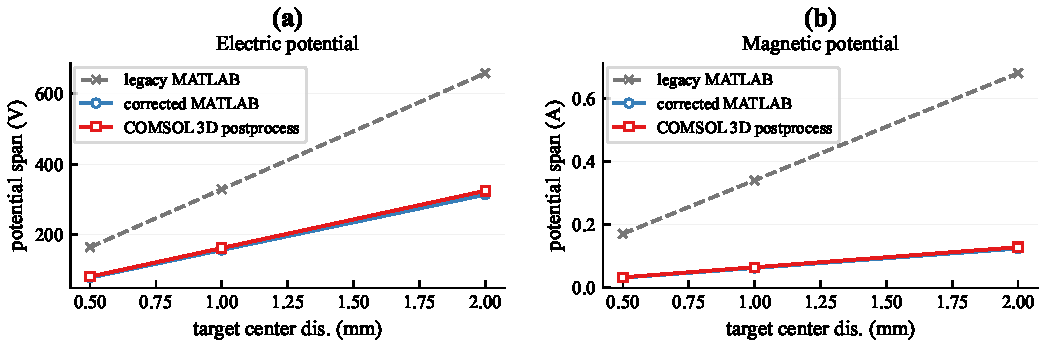
\includegraphics[width=0.94\textwidth]{Fig_02_inverse_sensor_correction.pdf}
\caption{旧 MATLAB、修正 MATLAB 与 COMSOL 三维力学--本构后处理的反传感结果。修正消除了十层重复热释耦合造成的量级膨胀。}
\label{fig:inverse}
\end{figure}

该 COMSOL 结果属于 B 级交叉验证：三维力学应变独立，但电势/磁势由同一冻结本构后处理，而非独立电磁 PDE 开路求解。因此可写“修正得到跨实现的 $3.47\%$ 一致性”，不能写“独立多物理场误差已小于 1\%”。

\section{曲率--功能梯度创新工况}

\subsection{计算覆盖与模板半径审计}

已完成平板与 $R=1.0,0.4,0.3,0.2$ m、U/X 两类梯度、力/电/磁三类载荷的 30 行筛选。早期一个标称 $R=0.4$ m 的 20$\times$20 模板经节点坐标反算实际为 $R=0.6$ m，已从网格收敛证据中排除；随后由平板节点重新生成真实 $R=0.4$ m、弧长 0.3 m 的 20$\times$20 案例。该审计避免了把几何不一致误报为网格误差。

\subsection{筛选趋势与代表点网格验证}

10$\times$10 筛选显示：随曲率增大，压力工况中心位移总体下降，在 $R=0.2$ m 时约为平板的 $0.79$；电致/磁致位移则在 $R=0.3$--$0.4$ m 附近达到平板的约 $1.20$--$1.22$。这给出了“曲率对外载荷弯曲与内禀致动响应方向不同”的可检验假设。

\begin{table}[H]
\centering
\caption{$R=0.4$ m、30$\times$30 代表点的梯度--曲率交互}
\small
\begin{tabular}{lrrrr}
\toprule
载荷 & U 曲率/平板 & X 曲率/平板 & 交互/百分点 & 最大 20$\to$30 变化 \\
\midrule
压力 & $0.921025$ & $0.920864$ & $-0.01606$ & $0.03982\%$ \\
电致 & $1.204941$ & $1.219624$ & $+1.46828$ & $0.02081\%$ \\
磁致 & $1.204941$ & $1.219624$ & $+1.46828$ & $0.02081\%$ \\
\bottomrule
\end{tabular}
\end{table}

压力交互仅为网格变化的 0.40 倍，不能判为已分辨；电致和磁致交互约为最大网格变化的 70.6 倍，可判为稳定的非加性交互。即曲率不仅统一缩放响应，还会改变 U/X 梯度对内禀致动的相对效果，这是当前最适合作为小论文创新主线的结果。

\begin{figure}[H]
\centering
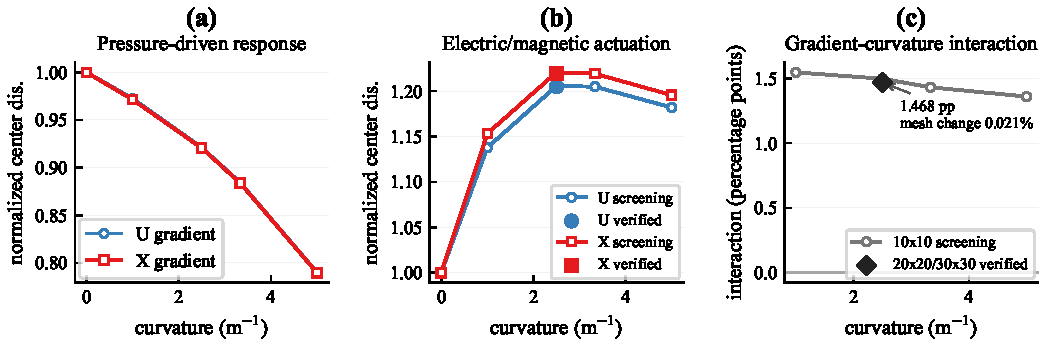
\includegraphics[width=0.98\textwidth]{Fig_01_curvature_gradient_interaction.pdf}
\caption{曲率--梯度响应：左、中为 10$\times$10 全半径筛选，右为 $R=0.4$ m 的 20$\to$30 网格验证。}
\label{fig:curvature}
\end{figure}

当前边界是：全半径曲线仍属于 10$\times$10 探索性筛选；只有 $R=0.4$ m 的 U/X 代表点完成了 20$\times$20 与 30$\times$30 高精度验证。因此可报告代表点交互，尚不应把整条半径曲线写成全部高精度参数图谱。

\section{验证门槛、论文可用结论与剩余必要工作}

\begin{table}[H]
\centering
\caption{截至 2026-07-15 的闭环状态}
\small
\begin{tabularx}{\textwidth}{p{0.25\textwidth}Xp{0.16\textwidth}}
\toprule
项目 & 已获证据与门槛判断 & 状态 \\
\midrule
力致平板基线 & 同口径主点已进入 1\% & \pass \\
300 V/200 A 直接 COMSOL & 两链均正常求解，场值与网格门槛通过 & \pass \\
直接场跨模型 1\% & 当前比较为 LRT5 板对三维实体，偏差 10.77\%/9.27\% & \na \\
反传感 MATLAB 装配 & 十层重复热释项已定位、修正并可回归复现 & \pass \\
反传感 COMSOL 交叉验证 & 20$\times$20 差异 3.4654\%，B 级、非完全独立 PDE & \pass \\
曲率--梯度筛选 & 30 行工况完整；趋势和候选半径已获得 & \pass \\
$R=0.4$ m 代表点 & U/X、三载荷完成 20/30 网格检查；致动交互已分辨 & \pass \\
全半径高精度图谱 & 除 $R=0.4$ m 外尚未逐点做 20/30 网格验证 & \wait \\
代表曲壳独立 COMSOL & 尚未建立严格同构的曲壳对照 & \wait \\
\bottomrule
\end{tabularx}
\end{table}

\subsection{现在可以用于小论文的表述}

\begin{itemize}
\item 20$\times$20 大偏差由网格导致的假设已被多组区分性试验否定，剩余差异主要是板理论与三维实体的模型形式差；
\item MATLAB 反传感旧结果存在可定位、可复现的十层热释耦合重复装配，修正后 0.5--2.0 mm 仍严格线性；
\item $R=0.4$ m 处，电致/磁致的 U/X 梯度--曲率交互约为 1.4683 个百分点，显著高于离散误差，而压力交互尚未分辨。
\end{itemize}

\subsection{投稿前仍属必要的内容}

\begin{enumerate}[label=\arabic*.]
\item \textbf{同构正向验证：}若保留“小于 1\%”表述，必须建立 COMSOL 分层壳或 MATLAB 三维实体同构对照；否则在论文中将当前直接场结果明确降级为模型形式敏感性验证。
\item \textbf{曲率主图加密：}对论文最终选用的半径点补做 20/30 网格复算；无需重新重复已经排除的场强、厚度网格和侧压力诊断。
\item \textbf{代表曲壳交叉验证：}至少选择 $R=0.4$ m 的 U/X 电致或磁致工况，建立匹配几何、边界和输出定义的独立模型。
\item \textbf{可复现性抽检：}对进入正文的平板、曲壳及反传感代表行保存输入哈希、日志、CSV 与绘图脚本版本。
\end{enumerate}

上述四项决定“可投稿”而非“当前阶段有没有结果”。目前已经形成可写的机制主线和经过网格验证的代表点，但尚不能把非同构的直接场对照写成近零误差，也不能把 10$\times$10 全半径筛选包装成完整高精度图谱。

\section{可复现证据索引}

\begin{longtable}{>{\raggedright\arraybackslash}p{0.31\textwidth}>{\raggedright\arraybackslash}p{0.63\textwidth}}
\toprule
证据 & 路径 \\
\midrule
\endfirsthead
\toprule
证据 & 路径 \\
\midrule
\endhead
20$\times$20 深入诊断 & \nolinkurl{outputs/paper-20260715-fgmee/experiments/deep_20x20_bias_diagnosis.md} \\
误差来源矩阵 & \nolinkurl{outputs/paper-20260715-fgmee/experiments/error_source_matrix.csv} \\
MATLAB 正向网格诊断 & \nolinkurl{outputs/paper-20260715-fgmee/experiments/results/matlab_forward_mesh_diagnostic.csv} \\
COMSOL 正向网格汇总 & \nolinkurl{outputs/paper-20260715-fgmee/experiments/direct_comsol_mesh_validation.csv} \\
COMSOL 电/磁正式结果与日志 & \nolinkurl{outputs/paper-20260715-fgmee/experiments/comsol/} \\
反向 COMSOL 驱动 & \nolinkurl{tools/comsol/RunInverseSensorCfffValidation.java} \\
反传感深度诊断 & \nolinkurl{outputs/paper-20260715-fgmee/experiments/inverse_sensing/inverse_sensor_deep_diagnosis.md} \\
修正前后/COMSOL 对比 & \nolinkurl{outputs/paper-20260715-fgmee/experiments/inverse_sensing/inverse_sensor_corrected_comparison.csv} \\
热释项十层审计 & \nolinkurl{outputs/paper-20260715-fgmee/experiments/inverse_sensing/inverse_pyro_overcount_audit.csv} \\
曲率--梯度 30 行筛选 & \nolinkurl{outputs/paper-20260715-fgmee/experiments/curvature_fg/curvature_fg_pilot_10x10.csv} \\
$R=0.4$ m 网格验证 & \nolinkurl{outputs/paper-20260715-fgmee/experiments/curvature_fg/curvature_fg_meshcheck_R0p4_final.csv} \\
曲率交互汇总 & \nolinkurl{outputs/paper-20260715-fgmee/experiments/curvature_fg/curvature_fg_displacement_interaction_final.csv} \\
几何半径审计 & \nolinkurl{outputs/paper-20260715-fgmee/experiments/curvature_fg/curvature_template_radius_audit.csv} \\
论文图绘制脚本 & \nolinkurl{tools/plotting/plot_stage2_publication_figures.py} \\
\bottomrule
\end{longtable}

\subsection*{AI 使用说明}
本报告由 AI 辅助核查本地 MATLAB/COMSOL 代码、模型、日志与 CSV，并生成 LaTeX 文档和论文图。所有数值结论均绑定上列本地证据。AI 未把非同构模型的差异改写为数值误差，也未将探索性筛选提升为全部高精度结论。

\end{document}
